\documentclass{scrreprt}
\usepackage[english]{babel}
\usepackage[T1]{fontenc}
\usepackage{lmodern}
\usepackage{blindtext}
\usepackage[utf8]{inputenc}
\usepackage{siunitx} %For unit handling%
\renewcommand{\familydefault}{\sfdefault}
\newcommand{\unit}[1]{\ensuremath{\, \mathrm{#1}}}
\usepackage{amssymb, amsmath, cancel, ulem, graphicx, float, tabularx, multirow, bm}
\usepackage{amsmath}
\usepackage{caption}
\usepackage{subcaption}
\usepackage{mathtools}
\usepackage{tikz}
\newcommand*\circled[1]{\tikz[baseline=(char.base)]{
            \node[shape=circle,draw,inner sep=1pt] (char) {#1};}}
\renewcommand{\phi}{\varphi}


\setcounter{secnumdepth}{5}
\setcounter{tocdepth}{5}

\author{Urs Gerber\\09-921-156 \and Gian-Luca Mateo\\11-113-545}
\date{18th of April 2013}

\title{Coupled pendulums}
\subtitle{Practical course report}

\begin{document}

\maketitle

\tableofcontents
\newpage

\chapter{Experiment: Coupled pendulums}

\section{Introduction}

\subsection{Goal of the experiment}
The goal of this experiment is to measure and analyse the characteristics of a coupled pendulum. For that we measure the cycle duration of the coupled pendulum in three different oscillation modes: in-phase, opposite in-phase and paraphase.

\subsection{Theory}

\subsubsection{Mathematical pendulum}
\paragraph{Equation of motion}
The equation of motion for the mathematical pendulum with thread length $l$ is given by
\begin{equation}
\ddot{\phi} + \frac{g}{l} \cdot \sin{\phi} = 0 \xRightarrow{\sin{\phi}\approx\phi} \ddot{\phi} + \frac{g}{l} \cdot \phi = 0
\end{equation}
with solution 
\begin{equation}
\phi (t) = \hat{\phi} \cdot \sin{\left( \sqrt{\frac{g}{l}} \cdot t + \phi_0 \right)} 
\end{equation}
The oscillation period $T_0$ of the mathematical pendulum is
\begin{equation}
T_0 = 2 \pi \sqrt{\frac{l}{g	}}
\end{equation}

\subsubsection{Coupled physical pendulum}

\paragraph{Equation of motion}
The equation of motion for one physical pendulum is given by

\begin{equation}
J\cdot \ddot{\phi} = M
\end{equation}
where $J$ is the moment of inertia with respect to the axis of rotation $O$ and $M$ the repulsive angular moment.

\paragraph{Moment equations}
The moment equations for pendulum 1 and pendulum 2 are:
\begin{align}
M_1 &= \overbrace{-D_g\cdot \phi_1}^{\text{directional moment}} + \overbrace{D_f \cdot (\phi_1 - \phi_2)}^{\text{coupling moment}}  \\
M_2 &= -D_g\cdot \phi_2 - D_f \cdot (\phi_1 - \phi_2)
\end{align}

After inserting the moment equations into the equation of motion and solving the differential equations, we get the two solutions

\begin{align}
\phi_1(t) &= A \cdot \cos{(\omega t + \delta)} - B \cdot \cos{(\Omega t + \Delta)}\\
\phi_2(t) &= A \cdot \cos{(\omega t + \delta)} + B \cdot \cos{(\Omega t + \Delta)}
\end{align}
with natural frequencies $\omega$ and $\Omega$
\begin{align}
\omega &= \sqrt{\frac{D_g}{J}}\\
\Omega &= \sqrt{\frac{D_g+2 D_f}{J}}
\end{align}
One can see that the overall motion of each pendulum is composed of a superposition of two harmonic oscillations with different frequencies (beat).

\paragraph{Initial values}
We distinguish the following three cases for pendulum 1 and pendulum 2. At $t=0$ the initial deflection of the pendulums may be
\begin{itemize}
\item in-phase: $\phi_1 = \Phi, \quad \phi_2 = \Phi$
\item opposite in-phase: $\phi_1 = -\Phi, \quad \phi_2 = +\Phi$
\item paraphase: $\phi_1 = 0, \quad \phi_2 = \Phi$
\end{itemize}

\subsection{Uncertainty analysis}

\section{Experiment setup and execution}

\subsection{Used materials}
The materials used in this experiment are the following:
\begin{itemize}
\item An assembly (labelled No.$3$) with two ball bearing mounted sticks ($21.37\unit{g}$ each), which have threaded bottoms
\item Two weights ($214.15 \unit{g}$ each) with threaded holes which can be screwed onto the bottom of the sticks and secured with two nuts ($2\unit{g}$ each)
\item two brackets, mountable to the sticks
\item a spring, attachable to the brackets 
\item a ruler, metric scale, $38 \unit{cm}$ long
\item a mechanical stopwatch, $0.2 \unit{s}$ steps
\end{itemize}

\subsection{Assembly}
For our measurements, the materials are assembled as shown in image \ref{fig:assembly}.

\begin{figure}[H]
	\centering
  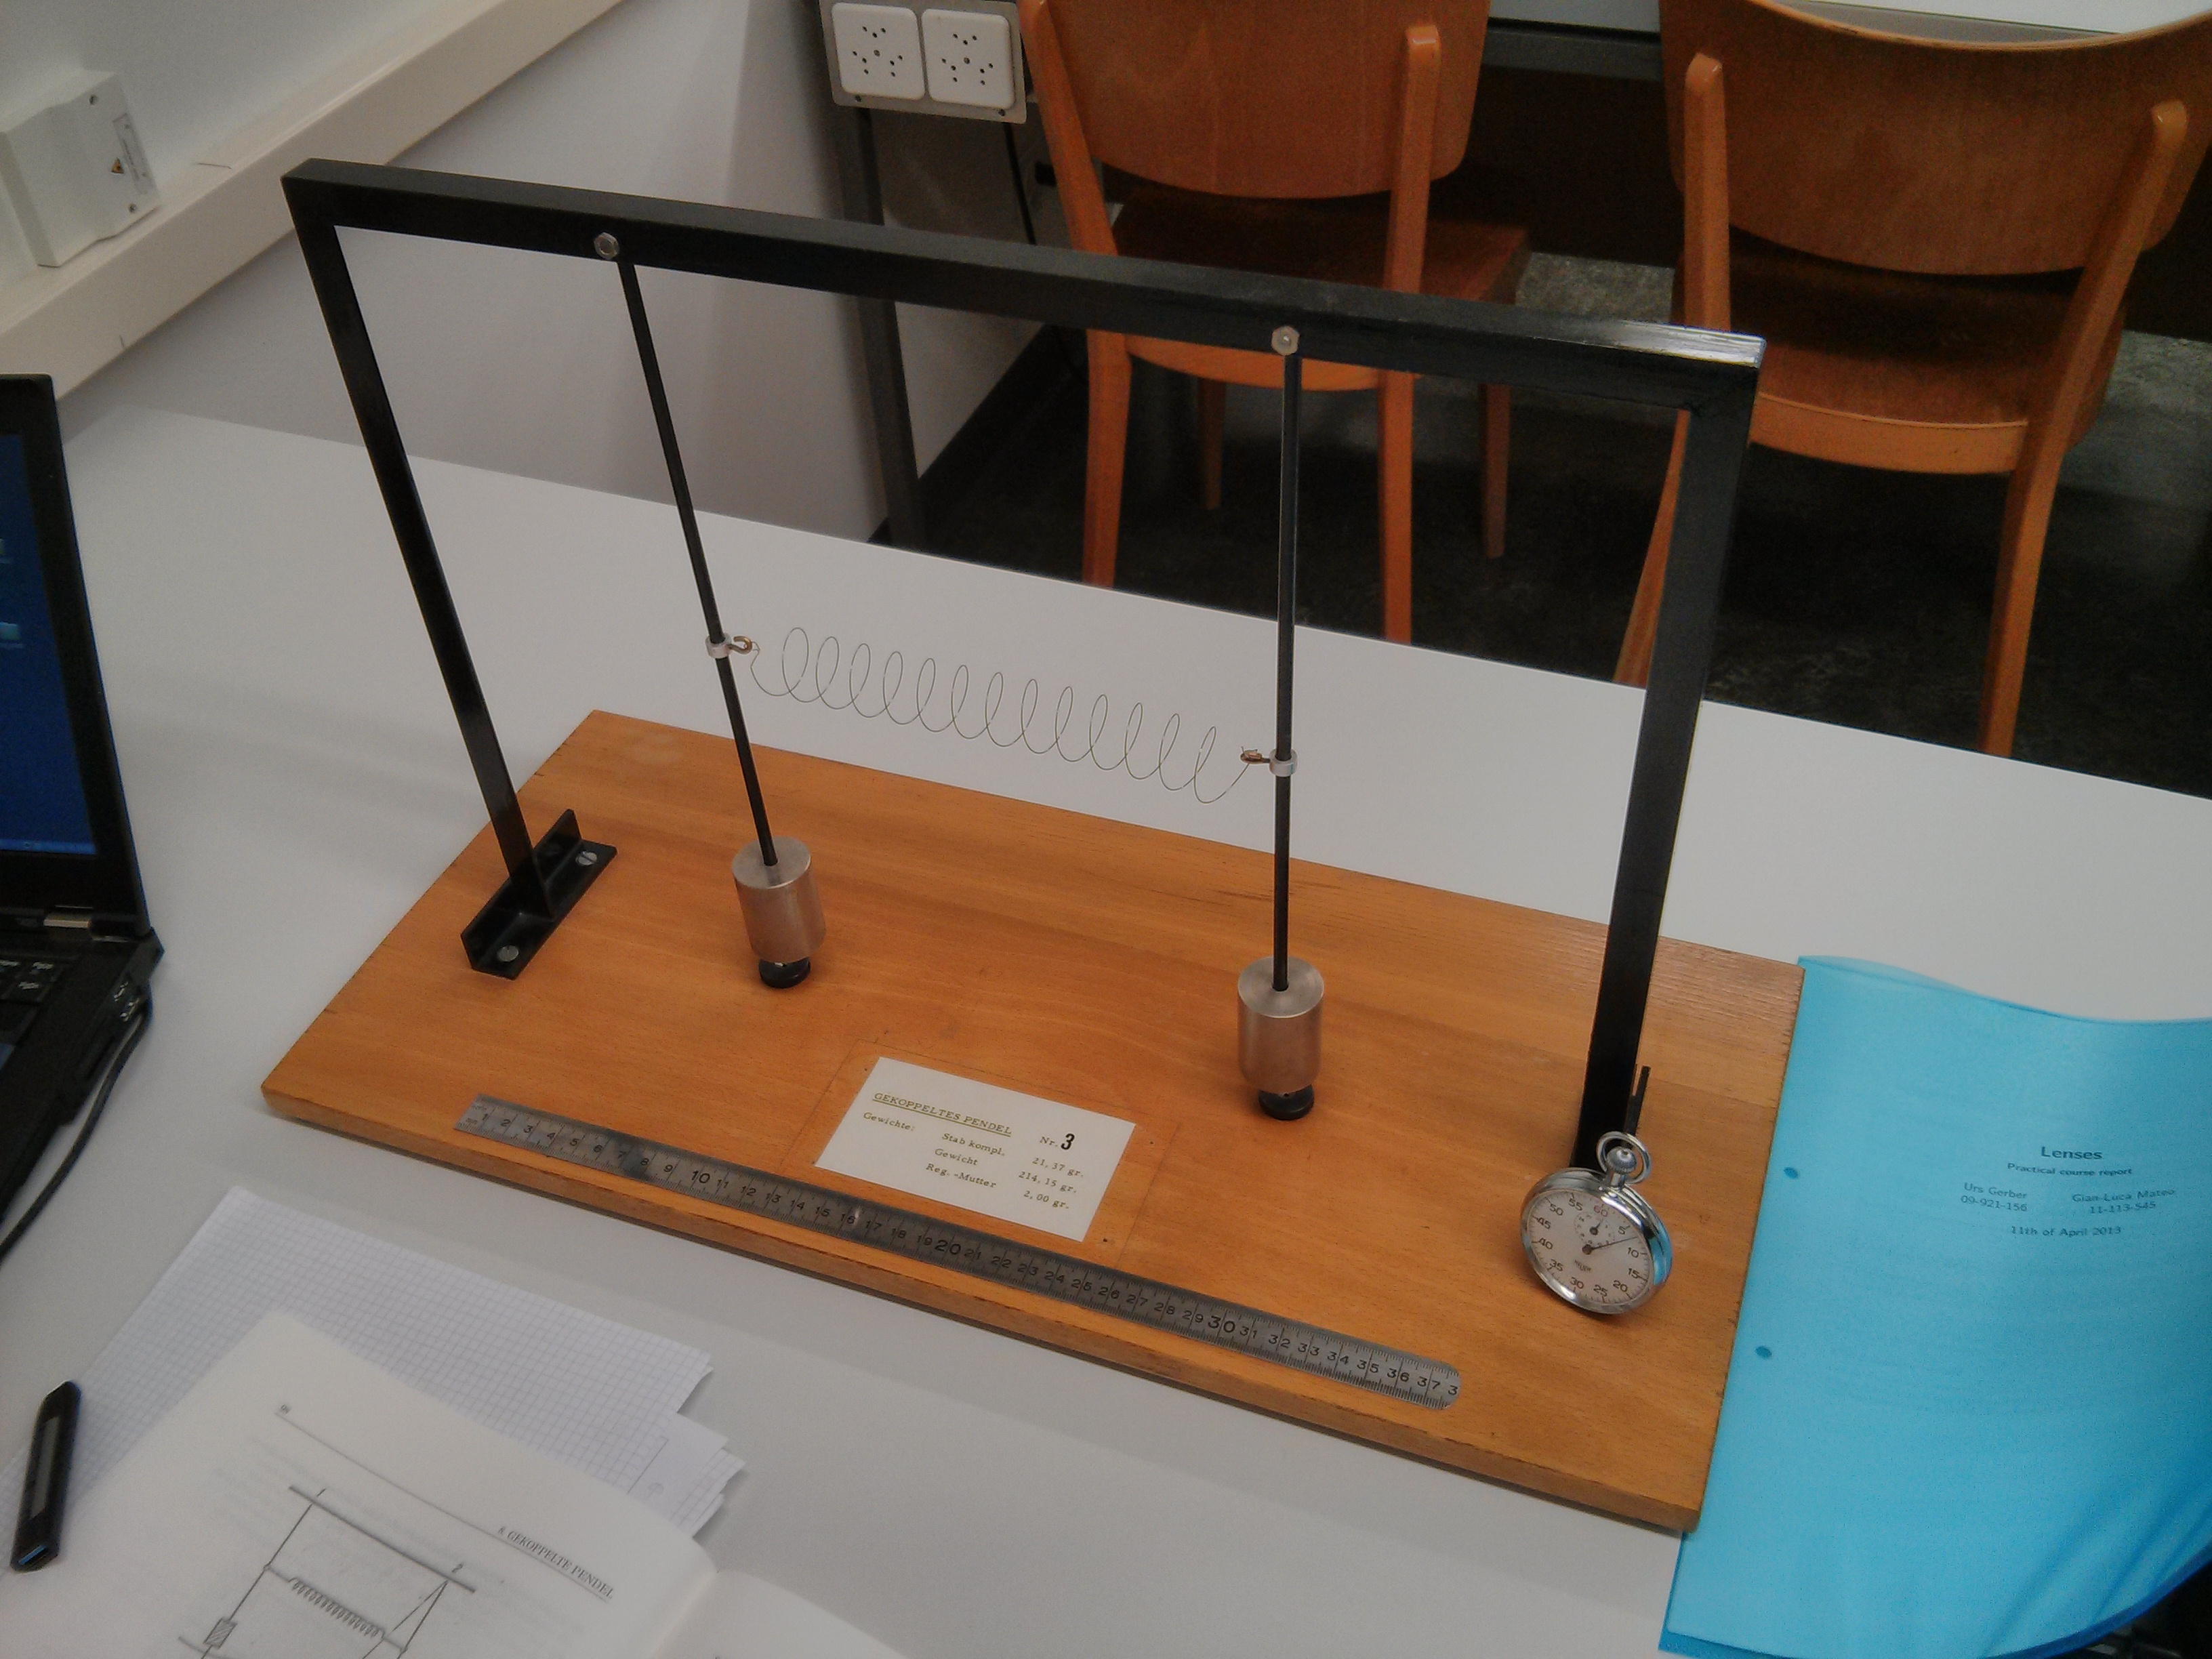
\includegraphics[width=0.9\textwidth]{img/assembly.jpg}
	\caption{Experiment Assembly}
	\label{fig:assembly}
\end{figure}
For the first series of measurements, one pendulum is detached from the spring, deflected and its oscillation period measured. for the second series, the weight at the bottom of the second pendulum is moved up or down in order to obtain the same period as the first one. Next, the spring is attached to both pendulums at the same height. Once this is done, the following values are measured:
\begin{itemize}
\item $\tau_{\omega}$: in-phase oscillation period, $\phi_1 = \phi_2$
\item $\tau_{\Omega}$: opposite in-phase oscillation period, $\phi_1 = -\phi_2$
\item $\tau$ : paraphase oscillation period, $\phi_1 = 0, \phi_2 = \Phi$
\item $T_s$ : beat period (the time spent between two stops of a pendulum)
\end{itemize}
\section{Measurements}

\begin{figure}[H]
	\centering
  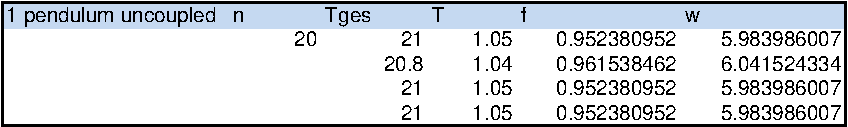
\includegraphics[width=0.9\textwidth]{diag/uncoupled.pdf}
	\caption{Measurements with the spring left unattached}
	\label{fig:uncoupled}
\end{figure}

\begin{figure}[H]
	\centering
  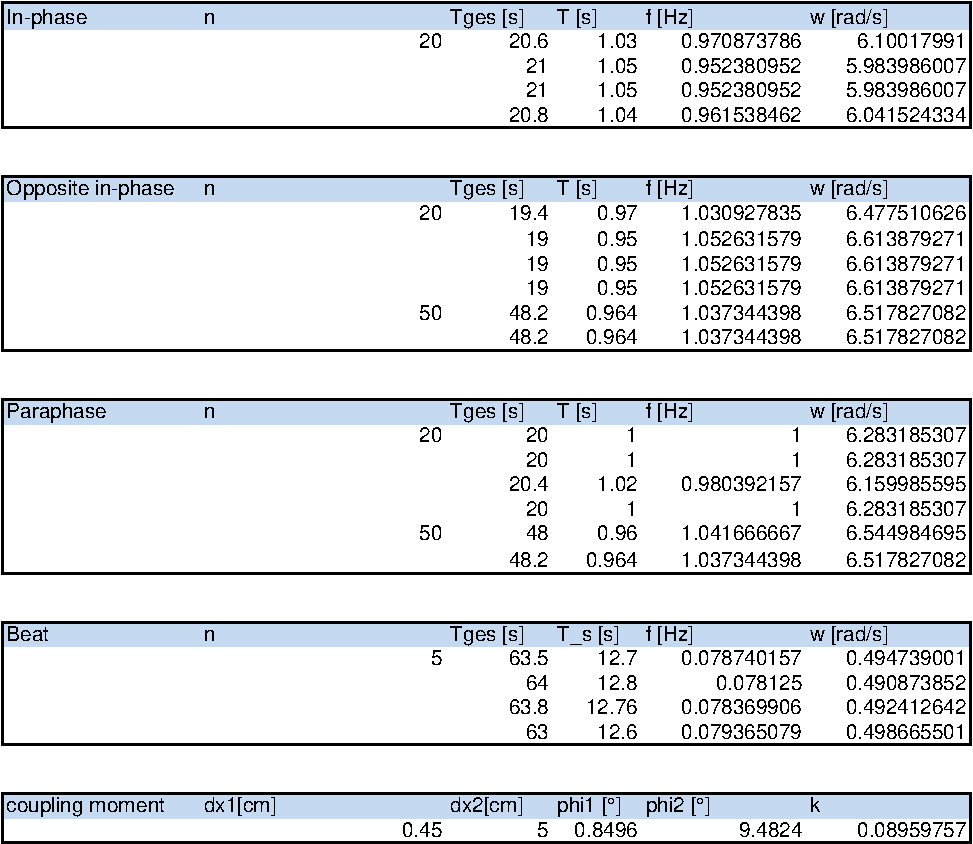
\includegraphics[width=0.9\textwidth]{diag/readings20cm.pdf}
	\caption{Measurements with the spring attached at $20\unit{cm}$ from the top}
	\label{fig:20cm}
\end{figure}

\begin{figure}[H]
	\centering
  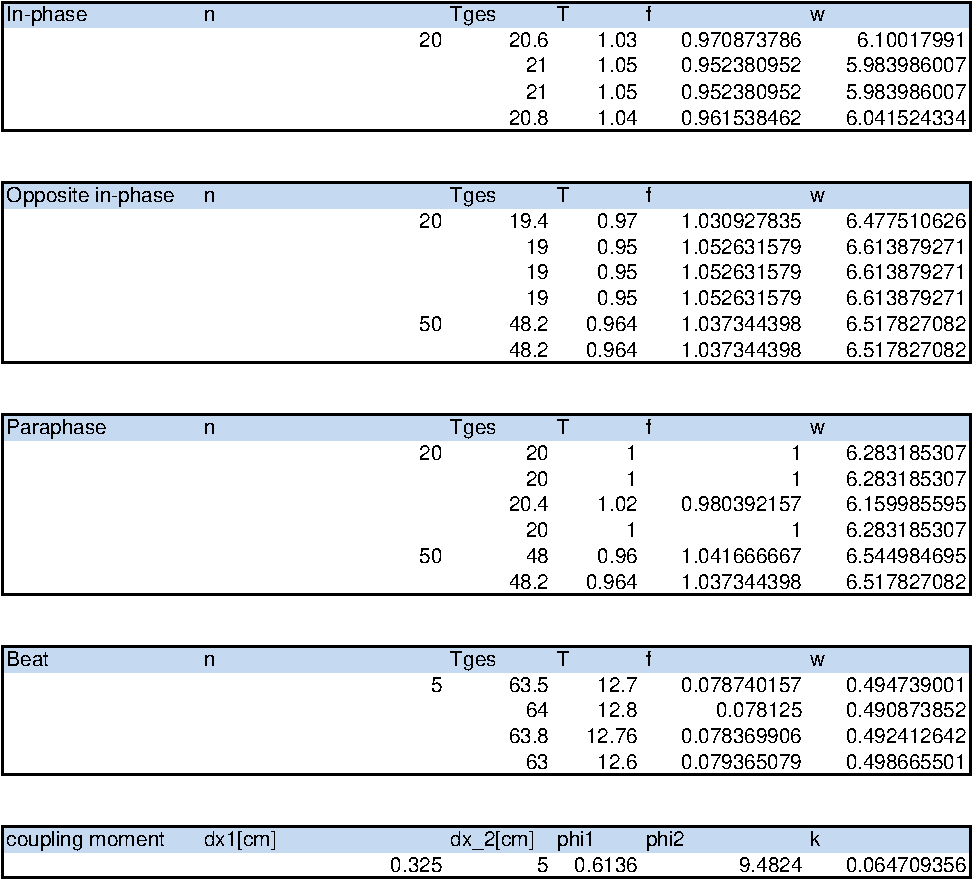
\includegraphics[width=0.9\textwidth]{diag/readings15cm.pdf}
	\caption{Measurements with the spring attached at $15\unit{cm}$ from the top}
	\label{fig:15cm}
\end{figure}
\begin{table}[H]
	\centering
	\begin{tabular}{|lcc|}
		\hline
		d&=&$27.2\unit{cm}$\\
		l&=&$30.35\unit{cm}$\\
		\hline
	\end{tabular}
	\caption{measured lengths of the pendulum}
\end{table}

\section{Analysis and Discussion}

\section{Conclusion}

\begin{thebibliography}{9}

\bibitem{physcript13}
  Peter Wurz,
  \emph{Anleitung zum Physikpraktikum}
  FS2013

\end{thebibliography}

\end{document}
